\chapter{\dunyazad/}

\label{ch:dunyazad}

As stated in the introduction, \dunyazad/ has two purposes as a project: first, to produce a \emph{system}, and second, to produce a \emph{theory}.
%
The system is a novel story generator that is focused on generating interesting choices, and on providing fine-grained control over the kinds of choices it uses.
%
The theory is a theory of choice poetics: a theory about how specific choice structures give rise to certain feelings, such as regret.
%
In order to satisfy these two goals, \dunyazad/ uses an answer set solver to turn a logical criteria for a certain kind of choice into an instance of such a choice--this it it's core operating principle.


\dunyazad/'s code therefore largely consists of a set of logical statements describing what a choice structure is and when choices fit into one of several categories.
%
For example, there are statements that define a ``relaxed'' choice.
%
Answer sets for these rules are found using Potassco Labs' \clingo/ solver \cite{Gebser2011}.
%
Besides these rules, there is an external control structure which invokes the solver repeatedly, generating multiple choices and connecting them into a story.
%
The focus of development so far has been on individual choices, but the capacity exists for \dunyazad/ to generate a full branching story.
%
Of course, there is also some imperative code for turning a logical choice structure into English text, in the form of a template-based generation system.
%
The English-generation code and the control code are both written in Python.


The goal of this chapter is to describe in detail how \dunyazad/ functions.
%
First, \cref{sec:dunyazad-asp-and-ctp} describes why \dunyazad/ uses answer set programming in a bit more detail, and how answer set programming (ASP) helps with the theory development goal.
%
\Cref{sec:dunyazad-choice-generation} then describes how \dunyazad/ generates individual choices, while \cref{sec:dunyazad-control} describes the higher-level control mechanism, and \cref{sec:dunyazad-english} describes the template-based English generation component.
%
Finally, \cref{sec:dunyazad-summary} summarizes the entire system and works through an example of how \dunyazad/ generates a choice from beginning to end.

%\section{Goals}

\section{ASP and Critical Technical Practice}
\label{sec:dunyazad-asp-and-ctp}

The idea of critical technical practice started as a call for technical practitioners (and especially AI researchers) to be more aware of the limits placed on their technical approaches by the central metaphors of their fields.
%
In Phil Agre's 1997 \work{Computation and Human Experience} he describes a process of critical examination to identify core metaphors and what those core metaphors marginalize, followed by an inversion that makes those marginalized concepts central \cite{Agre1997}.
%
This process can be used to drive innovation and find hidden limitations in a technical field by scrutinizing it using the tools of critical theory.


Normal AI practice identifies a motivating theory and then attempts to build a system that faithfully operationalizes that theory, taking the theory for granted as an immutable truth.
%
In contrast, critical technical practice seeks to question common assumptions before embarking upon technical projects that use non-standard assumptions, thereby broadening the technical field.
%
\dunyazad/ as a project takes this a step further and sees its driving theory (thoice poetics) as a \emph{product} of technical practice rather than a precursor to it, integrating theory development tightly with system development.
%
\dunyazad/ thus not only actively questions its own theoretical assumptions: it changes them as a matter of course and in fact uses difficulties encountered during technical development to guide these changes.


In order to jointly develop \dunyazad/ as a system and choice poetics as a theory, a special technical approach is required--this is where answer set programming comes in.
%
One could imagine choice-point generators constructed using many different technologies, from case-based reasoning to something as complicated as neural networks.
%
However, most of these would fail to achieve the level of \emph{transparency} required for the system to provide useful feedback to the underlying theory.
%
In a neural-network based approach, for example, it would be very difficult to understand which part of the underlying theory is responsible for a particular generated choice structure, and even more difficult to use experimental results to inform changes in the theory.
%
Answer-set programming as a technical approach is thus motivated by the goal of developing choice poetics along side a technical system for generating choices.


The reason that answer-set programming is useful for critical technical practice is that answer set programs consist of a series of logical statements which dictate which combinations of predicates are allowed in the output.
%
This means that every predicate in the output set can be traced back to a set of rules in the program which allowed it to be present.
%
Sometimes this process is laborious, as many rules may chain together to allow a predicate, but  ultimately, every aspect of an answer-set program's output can be analyzed to figure out which specific statements were responsible for its presence.
%
Furthermore, because those logical statements correspond directly to elements of the underlying theory, the relationship between that theory and the program's output is visible.

% TODO: Better example here?
As an example, \dunyazad/ has rules that define one way in which a choice can be obvious--by having exactly one option which suggests a positive outcome and one or more options all of which suggest negative outcomes.
%
Originally, the criterion that the other options must suggest negative outcomes was not present, but upon looking at generated choices, some clearly didn't fit an intuitive test for obviousness because of their inclusion of neutral options.
%
Identifying the inclusion of these neutral options as the problem was easy, and it was also clear from inspection of the code that without a clause in the definition of ``obvious'' prohibiting neutral options, they would be allowed.
%
The fix at the system level was the extra clause requiring that all options at an obvious choice except the ``correct'' option should suggest negative outcomes.
%
Of course, this was not only a change in the code, it was also a change in the theory, because \dunyazad/'s code is a direct operationalization of choice poetics.
%
Obvious choices don't just have ``only one good option,'' instead they have ``one option which stands out from the rest as significantly better.''


In contrast with many techniques that could be applied to the problem of generating choice points, answer-set programming uniquely enables a tight integration of system development with theory development.
%
The use of answer-set programming as a design choice is thus driven not only by considerations at the system level, but also at the project level: in order for \dunyazad/ to produce both a system and a theory, the use of answer-set programming is critical.
%
In \dunyazad/, answer-set programming supports the aims of critical technical practice by helping make the system's underlying assumptions clearly visible, and by making every change to the system suggest a parallel change to the theory that it implements.

% TODO: Use this mini-rant somewhere?
%In contrast, statistical techniques often hide such assumptions through their use of data which is assumed to be unbiased and universally representative.
%
%In fact, the data sets used to drive statistical artificial intelligence techniques often contain many assumptions, but examination of these is far from straightforward and is seen a peripheral to most technical projects if it is considered at all.


\section{Choice Generation}
\label{sec:dunyazad-choice-generation}

\dunyazad/ generates choices by solving a complicated logic problems.
%
These problems are set up so that any solution will take the form of a choice, and further constraints can dictate certain properties of that choice (for example, that it must be an obvious choice).
%
Broadly, \dunyazad/'s rules can be split into four categories:

\begin{itemize}
\item \textbf{Representational constraints} establish the basic elements that \dunyazad/ arranges to form choices and stories.
\item \textbf{Constituent constraints} define the most basic rules for configuring representative elements to construct choices and stories.
\item \textbf{Aesthetic constraints} carve out a region within the space allowed by the constituent constraints, excluding gibberish and other categorically undesirable configurations.
\item \textbf{Poetic constraints} make distinctions between different desirable configurations and are selectively activated to produce different kinds of choices.
\end{itemize}

To understand how \dunyazad/ functions, it is first necessary to understand \dunyazad/'s (rather limited) view of what a choice is, and how choices fit together to form stories.
%
These things are defined by representational and constituent constraints.


\subsection{Story Representation}


In \dunyazad/, a story is represented as a sequence of actions, each drawn from a pre-determined set.
%
Besides actions, each timepoint in a story has an initial state, which can include characters, items, and relations between them.
%
\dunyazad/ also has ``setups,'' which are used to establish interesting situations that motivate action.
%
This kind of representation is amenable to logical reasoning and similar to representations used in planning-based story generation systems.
%
It is sufficient to represent a wide variety of simple stories focused on action (as opposed to say, character growth or the development of relationships).
%
Luckily, many of the original Choose-Your-Own-Adventure books are focused on actions and consequences, and the format of choice-based narrative lends itself to such stories, because they give rise to interesting choices.


\subsubsection{States}

\dunyazad/'s representational constraints define predicates for ``instances,'' which may be either ``actors'' or ``items,'' as well as ``states'' (binary properties of an instance), ``properties'' (instance properties which can be multi-valued), and ``relations,'' (named directional instance-to-instance links).
%
Besides these things, which can change from one state to the next as a result of the outcomes of actions, instances can have timeless ``surface properties'' like a name, which is stored but cannot be changed by events in the story.
%
\Cref{fig:dunyazad-states} gives examples of each of these and \cref{fig:dunyazad-state-example} shows how they come together to describe a situation.


\begin{figure}[!t]
\centering
%\includegraphics[width=\textwidth]{fig/dunyazad-states.pdf}
TODO: HERE
\caption[\dunyazad/'s State Predicates]{Predicates used to describe states in \dunyazad/.}
\label{fig:dunyazad-states}
\end{figure}


The core states in \dunyazad/ describe the cast and any items or skills that those characters possess.
%
Beyond these states are a group of states that describe transient relationships which set the stage for action, these are called ``potentials.''
%
Potentials include things like \prq{knows\_gossip}{,} \prq{injured}{,} and \prq{threatening}{,} and each is classified as either a ``problem'' or an ``opportunity.''
%
Although these special potential states are represented using normal \prq{state}{,} \prq{property}{,} and \prq{relation}{} predicates, actions which get rid of them must specify whether each potential is \prq{resolved}{,} \prq{manifested}{,} or \prq{nullified}{.}
%
Additionally, extra predicates specify whether a potential is \prq{problematic\_for}{} one or more of the actors involved (for example, the \prq{injured} state is \prq{problematic\_for}{} any actor to which it is applied).


\dunyazad/ understands based on this information whether the action which eliminated a potential was good or bad for different characters.
%
For example, an action that \prq{resolves}{} an \prq{injured} state is good for the actor who was injured, and thus taking that action makes sense for that character.
%
States themselves thus directly encode some of the information used to decide which actions are viable.
%
This not only helps the system reason about motivation, but it also makes the design of actions and setups easier by providing a standard set of states that trigger certain actions.


\begin{figure}[!b]
\centering
%\includegraphics[width=\textwidth]{fig/dunyazad-states.pdf}
\fbox{%
\parbox{\textwidth}{
Scene: \vspace{0.5em}\\
\ind ``A merchant carrying some perfume is being threatened by bandits.'' \vspace{0.5em} \\
Representation: \vspace{0.5em} \\
\ind \parbox{0.9\textwidth}{ \tt
inst(actor,businessperson\_4). \\
inst(actor,tough\_3). \\
inst(item,treasure\_5). \\
property(type,inst(actor,businessperson\_4),merchant). \\
property(type,inst(actor,tough\_3),bandits). \\
property(type,inst(item,treasure\_5),perfume). \\
relation( \\
\ind has\_item, \\
\ind inst(actor,businessperson\_4), \\
\ind inst(item,treasure\_5) \\
). \\
relation( \\
\ind threatening, \\
\ind inst(actor,tough\_3), \\
\ind inst(actor,businessperson\_4) \\
). \\
surface\_property(name,inst(item,treasure\_5),"perfume").
}
}
}
\caption[\dunyazad/ State Example]{An example scene description using \dunyazad/'s internal representation, showing the most-relevant predicates. In real output, each of these predicates except the \prq{surface\_property}{} would be tied to a specific timepoint, and there would be many more \prq{surface\_property}{} predicates describing things like the name of each instance and whether it is plural or singular. Note that each instance is assigned a unique identifier that ends with a number.}
\label{fig:dunyazad-state-example}
\end{figure}


\Cref{fig:dunyazad-state-example} is not quite accurate, because \dunyazad/'s non-surface state predicates are never encountered raw.
%
Instead, they are wrapped in \prq{st(<timepoint>, <state>)}{} predicates, to define different states of the world for each timepoint in the story.
%
The timepoints in a story form a directed acyclic graph that branches out from a single root node.
%
The structure of this graph is defined using \prq{successor(<previous>, <option>, <next>)}{} predicates which specify that the result of choosing option \prq{<opt>}{} at timepoint \prq{<previous>}{} is the state designated \prq{<next>}{.}
%
The root timepoint is named \prq{root}{,} and each successor is named for its parent plus the number of the option that leads to it, so for example, if there were three options at the \prq{root\_2}{} node, they would lead to timepoints labelled \prq{root\_2\_1}{,} \prq{root\_2\_2}{,} and \prq{root\_2\_3}{.}
%
The timepoints do not necessarily form a tree, however: if two outcomes lead to identical states, as long as it would not form a cycle in the graph, \dunyazad/ may connect them to the same timepoint.


\subsubsection{Actions}

As mentioned above, timepoints in \dunyazad/ are connected by options.
%
Each option is associated with a single action, and arguments describe the details of that action (for example, the initiator and/or target).
%
If a timepoint has more than one option, it represents a choice to be made by the player, otherwise it is simply an event that happens.
%
Actions specify lists of outcome variables with values for each variable.
%
For each outcome variable that an action has, a single outcome value is assigned to each option that uses that action, thereby defining the entire impact of that option on the world state.
%
These assignments have a shorthand notation \prq{o(<variable>, <value>)}{} which indicates that the outcome variable \prq{<variable>}{} takes on the value \prq{<value>}.
%
\Cref{fig:dunyazad-action-example} shows an example where at timepoint \prq{root}{,} the action associated with option 1 is \prq{talk\_down}{,} with two outcomes: \prq{o(attitude, convinced)}{} and \prq{o(enraged, not\_enraged)}{}.

\begin{figure}[!t]
\centering
\fbox{%
\parbox{\textwidth}{
Option: \vspace{0.5em}\\
\ind ``You try to talk the bandits down.'' \vspace{0.5em} \\
Outcome: \vspace{0.5em}\\
\ind ``You talk to the bandits and convince them to back off.'' \vspace{0.5em} \\
Representation: \vspace{0.5em} \\
\ind \parbox{0.9\textwidth}{ \tt
\cg{at(root,} action(option(1), talk\_down)\cg{).} \\

\cg{at(root,} arg(option(1), asking, inst(actor, you))\cg{).} \\
\cg{at(root,} arg(option(1), listening, inst(actor, tough\_3))\cg{).} \\
\cg{at(root,} arg(option(1), victim, \\
\ind inst(actor, businessperson\_4))\cg{).} \\

\cg{at(root,} outcome(option(1), o(attitude, convinced))\cg{).} \\
\cg{at(root,} outcome(option(1), o(enraged, not\_enraged))\cg{).} \\

\cg{at(root,} consequence\_of(option(1), o(attitude, convinced), \\
\ind \_not, relation(threatening, \\
\ind \ind inst(actor, tough\_3), inst(actor, businessperson\_4)))\cg{).} \\
\cg{at(root,} consequence\_of(option(1), o(enraged, enraged), \\
\ind \_not, relation(threatening, \\
\ind \ind inst(actor, tough\_3), inst(actor, you)))\cg{).} \\

\cg{at(root,} consequence(option(1), \\
\ind \_not, relation(threatening, \\
\ind \ind inst(actor, tough\_3), inst(actor, businessperson\_4)))\cg{).}
}
}
}
\caption[\dunyazad/ Action Example]{An example of action representation in \dunyazad/. Note that even outcomes which do not occur (\prq{o(enraged, enraged)}{} in this case) have their potential consequences noted via \prq{consequence\_of}{} predicates, but only outcomes that do occur (as specified by the \prq{at(<timepoint>, outcome(option(<opt>), o(<outvar>, <outval>)))}{} predicates) have actual consequences. }
\label{fig:dunyazad-action-example}
\end{figure}


Each action thus has multiple possible outcomes.
%
For the \prq{talk\_down}{} action, there are theoretically four: the \prq{attitude}{} outcome variable has two exclusive values \prq{convinced}{} and \prq{unconvinced}{,} while the \prq{enraged}{} outcome variable has two more values: \prq{enraged}{} and \prq{not\_enraged}{.}
%
However, the definition of \prq{talk\_down}{} stipulates that the outcome \prq{o(enraged, enraged)}{} is only possible if the outcome \prq{o(attitude, unconvinced)}{} is also present, so there are only three possibilities:

\begin{enumerate}
  \item The target is convinced to calm down (\prq{o(attitude, convinced)}{} and \prq{o(enraged, not\_enraged)}), in which case they stop threatening whoever they were threatening.
  \item The target is unconvinced, and nothing changes (\prq{o(attitude, convinced)}{} along with \prq{o(enraged, not\_enraged)}).
  \item The target is unconvinced, and gets mad at the person who tried to convince them (\prq{o(attitude, convinced)}{} along with \prq{o(enraged, enraged)}).
\end{enumerate}

Note that for a traditional planning system, because each combination of outcome variables has a different effect on the world state, each action would have to be broken into multiple sub-actions with fixed pre- and post-conditions.
%
The advantage of grouping them together conceptually is that this represents the player's view of things: the text introducing an option doesn't indicate the values of its outcome variables, and so the player can never be completely sure what outcomes an action will have.
%
This way of representing actions thus helps the system reason about how the player might perceive actions, this is the same reason that possible but unrealized state changes are explicitly represented by the system using \prq{consequence\_of}{} predicates (see \cref{fig:dunyazad-action-example}).


\begin{table}[!h]
\begingroup
\renewcommand*{\arraystretch}{1.5}
\begin{tabular}{c c c c}
  \pr{accuse}       & \pr{explain\_innocence} & \pr{play\_song}         & \pr{talk\_down} \\
  \cg{\pr{arrive}}       & \pr{flee}               & \pr{polymorph}          & \pr{tell\_story} \\
  \pr{attack}       & \pr{gossip}             & \cg{\pr{pursue}}             & \pr{trade} \\
  \pr{buy\_healing} & \pr{leave}              & \pr{reach\_destination} & \pr{travel\_onwards} \\
  \pr{deny\_blame}  & \pr{pacify}             & \pr{shift\_blame}       & \pr{treat\_injury} \\
  \pr{dispel}       & \pr{pay\_off}           & \pr{steal}
\end{tabular}
\endgroup
\caption[List of Actions in \dunyazad/]{The 23 actions currently defined in \dunyazad/. The \prq{arrive}{} and \prq{pursue}{} actions aren't currently used because the system has no setups that motivate them.}
\label{tab:dunyazad-action-list}
\end{table}


Besides defining outcomes, actions also define how skills affect their outcomes, but asserting that certain outcome values are linked to the presence or absence of particular skills on the part of one or more participants of the action.
%
Tools may also be involved.
%
For example the \prq{attack}{} action has an outcome variable \prq{success}{} with three values: \prq{victory}{,} \prq{defeat}{,} and \prq{tie}{.}
%
It specifies that the outcomes \prq{o(success, victory)}{} and \prq{o(success, defeat)}{} are both linked to the \prq{fighting}{} skill as alternate outcomes of a skill contest between the \prq{aggressor}{} and \prq{target}{} of the action, where tools are advantageous.
%
This means that if the aggressor of an attack action has both the \prq{fighting}{} skill and a tool for that skill, while the target of the attack has neither (or even if they're just missing a tool) the \prq{o(success, victory)}{} outcome is more likely, and the \prq{o(success, defeat)}{} outcome is less likely (the exact consequences of these assignments will be discussed in \cref{sec:dunyazad-poetic-constraints}).
%
Effectively, the definition of an action thus includes enough information for \dunyazad/ to consider both possible consequences of an action and what initial states might best foreshadow each different outcome.


\dunyazad/ currently has a total of 23 different actions, listed in \cref{tab:dunyazad-action-list}.
%
Given the setups that exist, however, the \prq{arrive}{} and \prq{pursue}{,}, actions are never motivated and thus impossible to use, so there are effectively 21 possible actions.
%
Most actions have at least two possible outcome configurations, and a few (such as \prq{attack{}}) have four or more.
%
However, the number of actions that are possible in a given state are limited by the constituent and aesthetic constraints.
%
This is where the setups come in: most actions require some sort of motivating state to make sense (the \prq{talk\_down}{} action, for example, requires that either a \prq{threatening}{} or an \prq{accusing}{} relationship be present).
%
Setups represent existing situations that the player might encounter while travelling, and each sets up conditions for a particular subset of actions.


\subsubsection{Setups}

Besides the initial state of the world having to do with the protagonist(s) and their starting skills and equipment, most of the state in \dunyazad/ comes from setups.
%
The situations \dunyazad/ creates are designed to fit into an overarching travel narrative: the protagonist(s) are on a journey, and encounter various obstacles.
%
This provides an excuse to repeatedly clean up the world state by having the main character(s) ``travel onwards,'' getting rid of any states except those pertaining to the main character(s) and introducing a new setup.
%
When putting multiple timepoints together into a complete branching story, \dunyazad/ starts by introducing a setup and then adding a few timepoints which resolve any outstanding potentials in that setup.
%
It then adds a \prq{travel\_onwards}{} option to each branch where potentials have been resolved, and adds a new setup to the timepoint that follows this option.


Setups are thus expected to set the stage for action: they provide a situation that contains the potential for something interesting to occur.
%
Some setups are quite flexible while others are specific.
%
For example, the \prq{healer}{} setup simply adds an actor with the \prq{healing}{} skill and a tool for healing who is offering to treat injuries for a price; it may only be used when a protagonist is injured.
%
In contrast, the \prq{market}{} setup potentially includes a lowlife, a healer, a laborer, an aristocrat, and up to two merchants.
%
These characters can have several potentials between them: the lowlife can be threatening one of the merchants, the noble might be accusing the peasant or one of the merchants, or perhaps the merchants are simply selling things and the noble or laborer knows some gossip.
%
The wide range of possibilities allowed by the \prq{market}{} setup lets \dunyazad/ create a variety of situations in service of creating particular choice structures, whereas the \prq{healer}{} setup is designed to be deployed in a very particular circumstance.
%
Although the \prq{market}{} setup eclipses the \prq{healer}{} setup in terms of actions enabled, the \prq{healer}{} setup's lack of extraneous characters provides a very different feeling to the player, and its surface text is more specific.


As mentioned above, not every timepoint includes setup-induced state changes: they only occur for the \prq{root}{} node and for timepoints that follow \prq{travel\_onwards}{} actions.
%
Internally, \dunyazad/ refers to everything that occurs between one setup and the \prq{travel\_onwards}{} events which follow that setup on each branch from it as a `vignette.'
%
The states associated with a setup are introduced after the \prq{travel\_onwards}{} action first removes all states associated with the old location--only states directly associated with a protagonist (such as an injury sustained or an item acquired) are retained.
%
Because \dunyazad/ effectively solves entire timepoints at once, however, the particular configuration of a setup's flexible elements can be changed at the same time that the actions, arguments, and outcomes of options are being decided.
%
This means that \dunyazad/ has the freedom to consider all possible setups as well as all configurations of actions given those setups when trying to build a particular choice structure, unless a certain setup is mandated by outside restrictions.


\subsection{Constituent Constraints}

\dunyazad/'s representation of stories as a graph of timepoints leaves lots of room for structures that don't make any sense.
%
This is where the constituent constraints come in.
%
While the basic predicates that define representational elements ensure things like continuity of states between timepoints, constituent constraints help ensure that actions get assembled into a story, instead of just a random sequence of unrelated events.
%
For example, rules that prohibit the same action from happening twice in a row,
or that require that each action be motivated, are constituent constraints.


While there is sometimes a gray area between constituent and aesthetic constraints, constituent constraints can often be identified as being concerned with getting \dunyazad/ to produce stories at all, while aesthetic constraints help defined \dunyazad/'s particular flavor of story.
%
If constituent constraints are removed, the results are often nonsensical; if aesthetic constraints are removed results still make sense, but they no longer fit with other stories that \dunyazad/ constructs.
%
\Cref{tab:dunyazad-constraints-inventory} lists all of the source code files from \dunyazad/'s main answer set problem definition code and briefly indicates what rules each file contains from each constraint type.

\begin{table}[!p]
\begin{minipage}[t]{\dimexpr0.5\textwidth-2em}
  \pr{actions.lp} \\
  \ind [representational] The association between actions and options; argument and outcome binding; consequences based on outcomes. \\
  \ind [constituent] Limits to interactions with incapacitated/off-stage actors. \\
  \ind [poetic] Definition of `surprising' outcomes based on likely/unlikely outcomes. \vspace*{0.5em} \\
  \pr{actors.lp} \\
  \ind [representatonal] Unpacking for actor definitions; top level of the actors ontology. \vspace*{0.5em} \\
  \pr{choice\_structure.lp} \\
  \ind [constituent] Motivation and relevance of options; bans redundancy, boredom, and repetition; encourages setup variety.  \\
  \ind [aesthetic] Enforces narrative perspecive (second-person); bans trick options. \\
  \ind [poetic] Story length and choice frequency constraints. \vspace*{0.5em} \\
  \pr{core.lp} \\
  \ind [representational] Basic structure definitions (options, events, choices, etc.); exclusivity for states; reflexivity for actions; ontology basics (inheritance). \vspace*{0.5em} \\
  \pr{eval.lp} \\
  \ind [poetic] Expectations; perceived and actual stakes; option feels; option structures; outcome perceptions; outcome predictabilities; outcome feels. \vspace*{0.5em} \\
  \pr{goals.lp} \\
  \ind [poetic] Player goals; apparent guilt of characters. \vspace*{0.5em} \\
  \pr{grow.lp} \\
  \ind [representational] Timepoint ordering and links; timepoint creation and state transfer; state matching. \vspace*{0.5em} \\
  \pr{items.lp} \\
  \ind [representational] Unpacking for item definitions; tool possession for a skill; communal ownership for trading. \vspace*{0.5em} \\
\end{minipage}%
\hfill
\noindent
\begin{minipage}[t]{\dimexpr0.5\textwidth-2em}
  \pr{potential.lp} \\
  \ind [representational] Resolution methods, initiators, urgency/immediacy, and importance of potentials; unresolved and hidden potentials. \vspace*{0.5em} \\
  \pr{settings.lp} \\
  \ind [content] The possible settings. \\
  \ind [representational] Assignment of settings to timepoints; setting continuity and changes. \vspace*{0.5em} \\
  \pr{setup.lp} \\
  \ind [representational] Unpacking setups; creating/editing associated states. \vspace*{0.5em} \\
  \pr{skills.lp} \\
  \ind [content] The list of skills (but skill-action links are specified by actions). \\
  \ind [representational] \vspace*{0.5em} \\
  \pr{surface.lp} \\
  \ind [representational] Surface properties like names and genders. \vspace*{0.5em} \\
  \pr{the\_party.lp} \\
  \ind [content] Rules that define the starting state of the protagonist(s). \vspace*{0.5em} \\
  \pr{vignettes.lp} \\
  \ind [constituent] Scoping of vignettes (actions in a single location). \vspace*{0.5em} \\
  \pr{content/*} \\
  \ind [content] These define the actions, goals, potentials, and setups that \dunyazad/ can use, along with its ontology of actors and items.
\end{minipage}
\caption[\dunyazad/ Constraints Inventory]{An inventory of \dunyazad/'s constraints organized by file and constraint type.}
\label{tab:dunyazad-constraints-inventory}
\end{table}

\subsection{Aesthetic Constraints}

\subsection{Poetic Constraints}
\label{sec:dunyazad-poetic-constraints}

\section{High-Level Control}
\label{sec:dunyazad-control}

\section{English Generation}
\label{sec:dunyazad-english}

\section{Summary}
\label{sec:dunyazad-summary}
